\section{Evaluation Results} \label{section_results}

Our XG-PON module is designed for simulating a 10Gbps optical
network with hundreds of ONUs and the simulation performance is
one of the most important metrics for researchers. Thus, in this
section, we will evaluate its simulation speed and memory
consumption under various scenarios with one off-the-shelf server.
Extensive pressure tests are also carried out to demonstrate our
XG-PON module can run for a very long time and work correctly
under more random simulation settings.

\subsection{Simulation Performance}

To avoid interference from other processes, one dedicated computer
is used to measure the performance of our XG-PON module. The
server used by us is Dell PowerEdge R320 rack server. The
processor is Intel(R) Xeon(R) CPU E5-1410 0 @ 2.80GHz and its
cache size is 10MBytes. Note that although this processor has 4
cores, just one of them is used by our simulation. As for the main
memory, the server is installed with 48GBytes in total.

\begin{figure}[!htbp]
\begin{center}
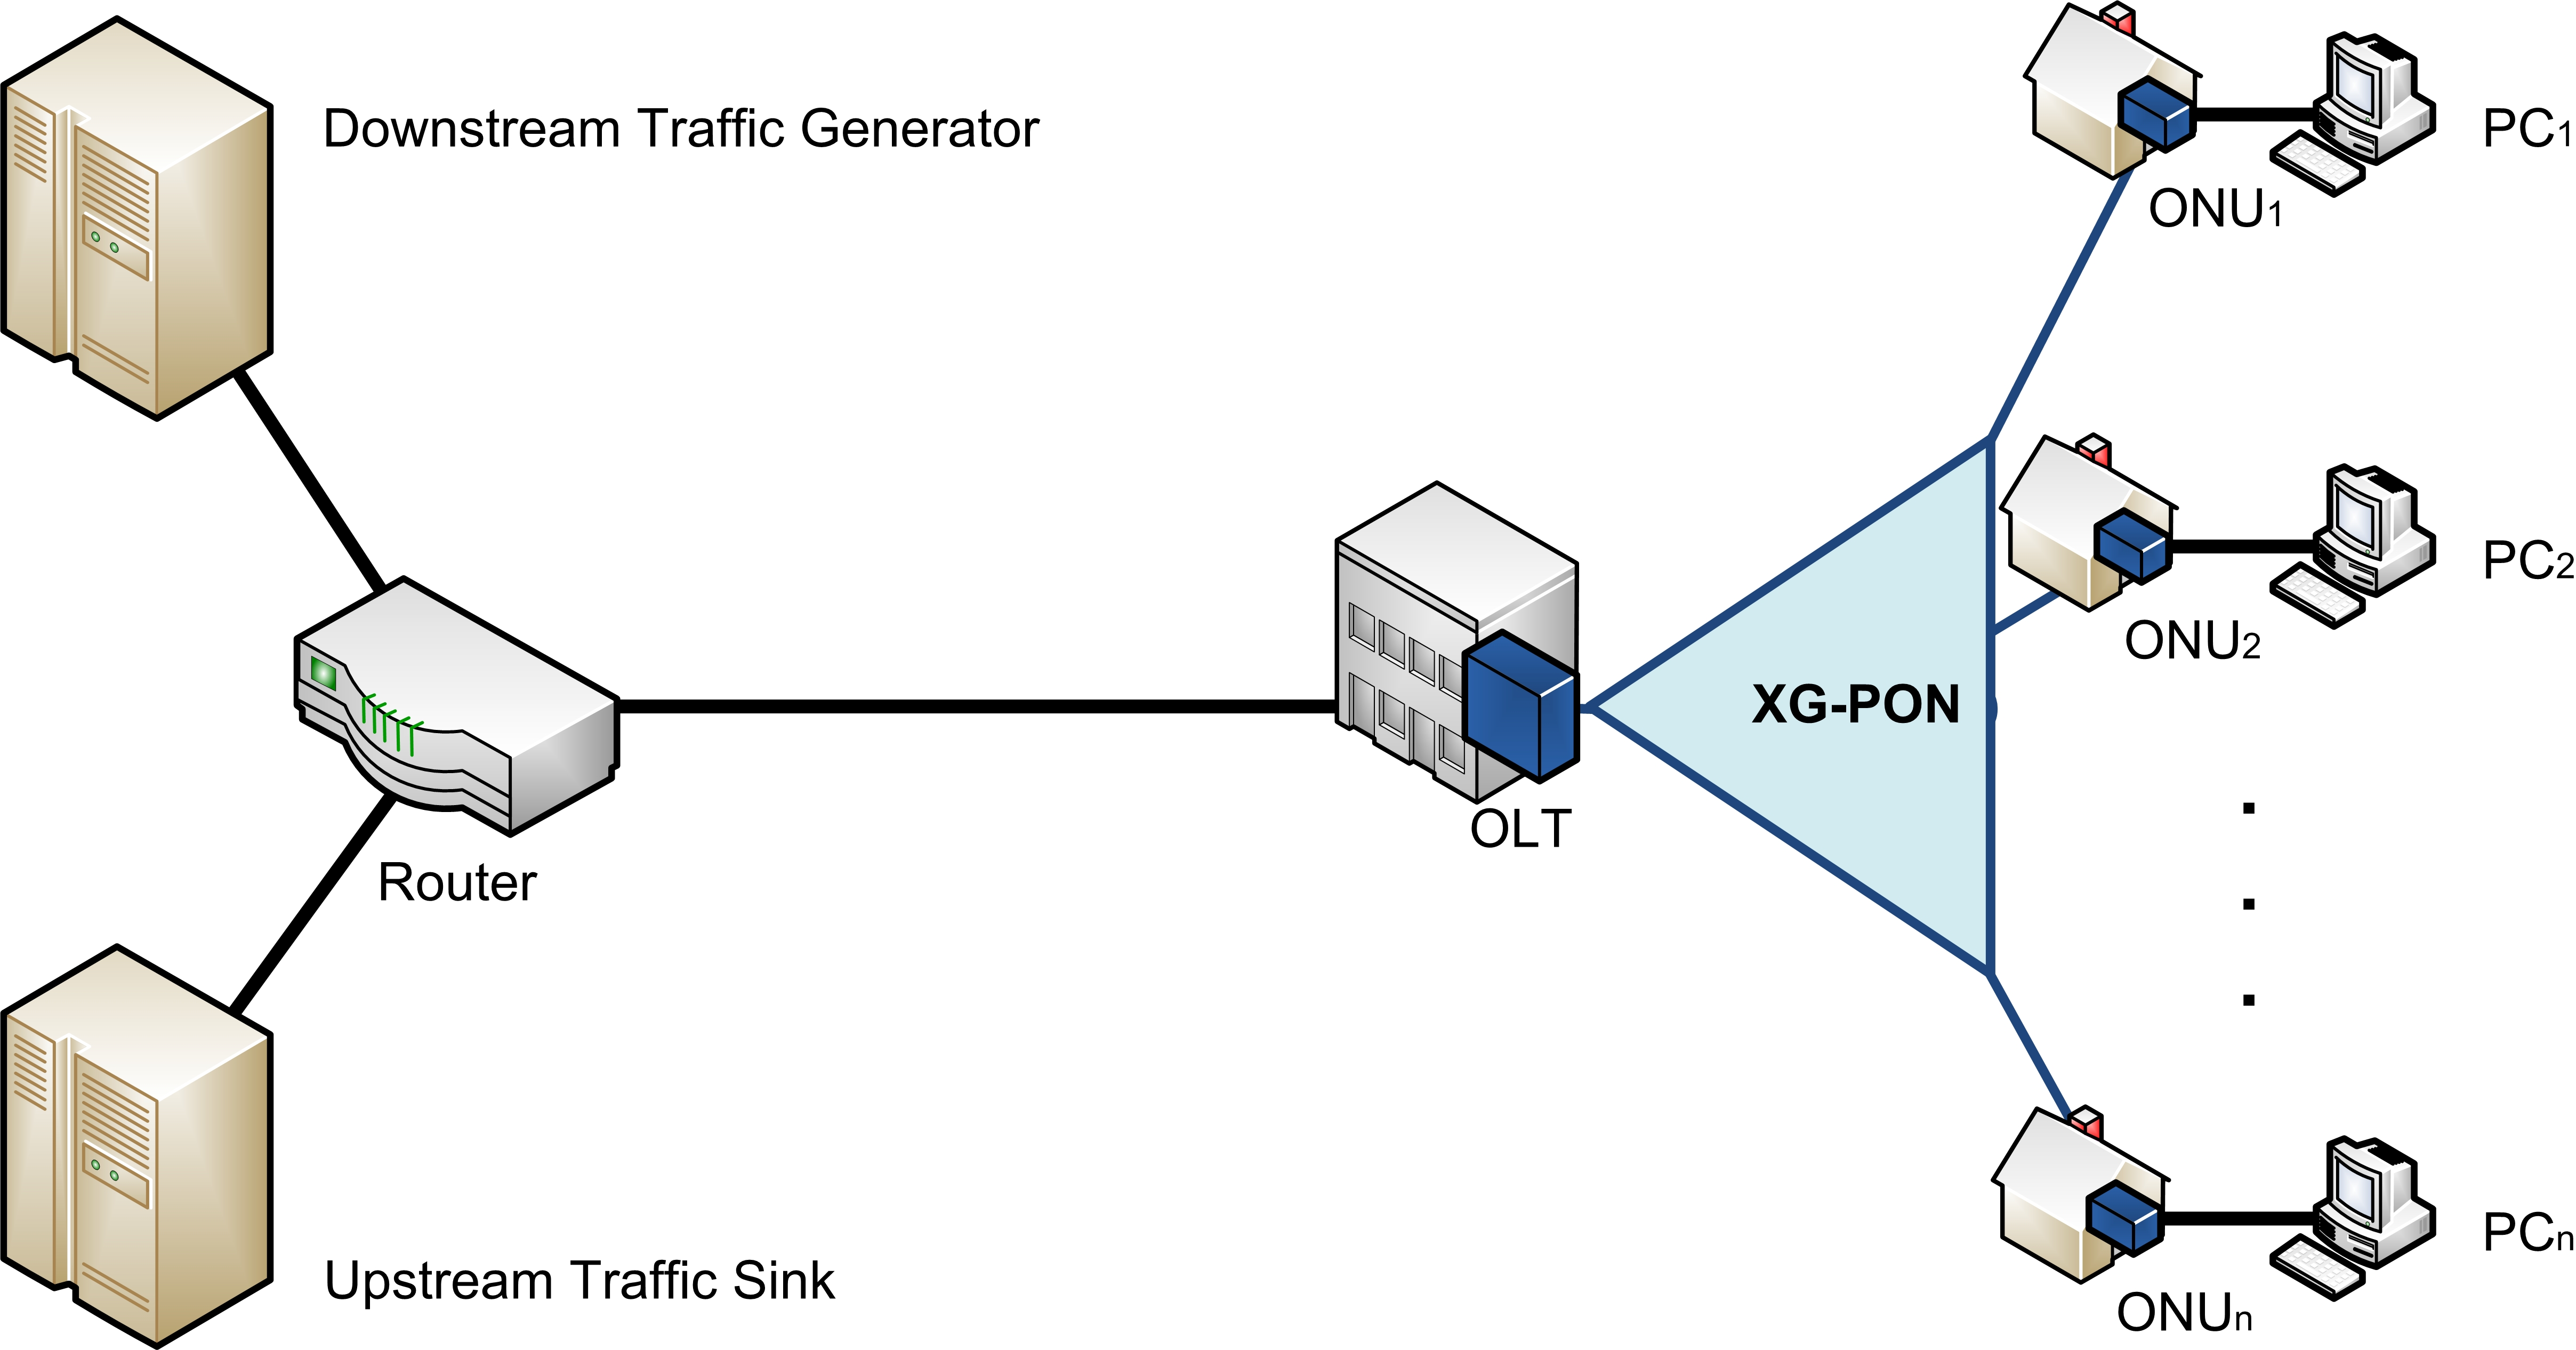
\includegraphics[width=0.75\textwidth]{images/topology}
\end{center}
\vspace{-0.1in}
\caption{Network Topology}
\label{fig_topology}
\end{figure}

The network topology used in our simulations is illustrated in
Figure \ref{fig_topology}. We simulate one XG-PON network whose
largest propagation delay is 0.4ms, i.e., the physical reach is
around 60km. For the data rates of XG-PON, we follow XG-PON1,
i.e., 10Gbps in downstream and 2.5Gbps in upstream. There are
totally $N$ ONUs in the XG-PON and one PC is connected to each ONU
through a point-to-point link whose delay is 2ms. These PCs act as
the customer of XG-PON and play the generators for the upstream
traffic and the sinks for the downstream. The OLT is connected to
Router and the point-to-point link between them is used to
simulate the core network. More specifically, the delay of this
link is set to 10ms. Downstream Traffic Generator and Upstream
Traffic Sink are connected to Router through point-to-point links
whose delay is 2ms. To generate network traffic in both
directions, each PC sends UDP packets to Upstream Traffic Sink and
receives UDP packets from Downstream Traffic Generator. Due to the
bandwidth asymmetry of XG-PON1, the generated data rate in the
upstream direction is always one quarter of the data rate in the
downstream direction. For all of the above point-to-point links,
the bandwidth is set to 20Gbps so that XG-PON is the only
bottleneck.

To study the simulation performance of our XG-PON module under
various scenarios, the number of ONUs and the amount of network
traffic are changed in our experiments. The evaluated values of
$N$ (the number of ONUs) are  25, 50, 100, 200, 400, 800, and
1000. As for the total amount of network load the downstream, the
evaluated values are, 150Mbps, 300Mbps, 600Mbps, 1.2Gbps, 2.4Gbps,
4.8Gbps, and 9.6Gbps. Note that due to the overhead of XG-PON
physical and XGTC layers, packets start to be dropped when the
downstream network load is 9.6Gbps. Furthermore, for all
experiments, the upstream network load is always one quarter of
the downstream network load. Thus, when the downstream network
load is 9.6Gbps, the upstream network load is 2.4Gbps and there
are also packets dropped in the upstream direction.



\begin{figure}[!htbp]
\vspace{-0.5in}
\begin{center}
\begin{tabular}{c} \vspace{-0.2in}
\subfigure[The amount of time consumed to simulate one second]{\label{fig_performance:speed}\includegraphics[width=0.6\textwidth,
angle=-90]{images/sim-udp-cpu.eps}} \\
\subfigure[The amount of memory consumed in steady phase]{\label{fig_performance:memory}\includegraphics[width=0.6\textwidth,
angle=-90]{images/sim-udp-mem.eps}}
\end{tabular}
\end{center}
\vspace{-0.1in}
\caption{Simulation Performance of XG-PON Module under Various Scenarios} \label{fig_performance}
\end{figure}

To evaluate the speed of our XG-PON module, 400 seconds are
simulated in each experiments, the total amount of time used to
complete the simulation is recorded, and we then calculate and
plot the amount of time consumed to simulated one second. Figure
\ref{fig_performance:speed} shows the results under various
scenarios. It indicates that the consumed time is increased
linearly with the network load. It is reasonable since NS-3 is one
packet-level network simulator and the number of events are
increased linearly with the number of packets. Figure
\ref{fig_performance:speed} also indicates that the consumed time
increases with the number of ONUs much slower. Hence, our XG-PON
module have successfully avoid to let each ONU process all packets
in the downstream direction. Figure \ref{fig_performance:speed}
also indicates that our XG-PON module takes around 160s to
simulate one second even when there are 1000 ONUs and the
downstream network load is 9.6Gbps with which XG-PON has been
over-loaded.

We have also used $gdb$ to run the simulation of the most 
difficult scenario (ONUs: 1000; Network load: 9.6Gbps) in $debug$ mode.
After the simulation enters into steady phase, we break it at random time, 
check the call stack, and continue the simulation. These steps are repeated 
for 126 times and the CPU is running our XG-PON code for only 4 times. 
Thus, our XG-PON module is not the bottleneck for simulation speed 
and other modules (routing, etc.) need be revised for improving 
the speed further.



Not only simulation speed, we have also evaluated the amount of memory
consumed by XG-PON simulation. The same experiments are repeated
to collect these results. For each experiments, after starting the
simulation, we wait for a long time until the simulation enters
into its steady phase and the amount of consumed memory does not
increase anymore. These values for various scenarios are recorded
and plotted in Figure \ref{fig_performance:memory}. This plot
indicates that the consumed memory increases linearly with the
network load, and it increase much slower with the number of ONUs.
When there are 1000 ONUs and the downstream network load is
9.6Gbps, the consumed memory is still less than 5GBytes.


In summary, with off-the-shelf servers, our XG-PON module can
simulate a 1000 ONUs 10Gbps XG-PON network with reasonable speed
and moderate memory consumption.


\clearpage

\subsection{Pressure Tests}

To evaluate the robustness of our XG-PON module, we have carried
out more experiments. In one group of experiments, we use the same
configurations designed for performance evaluation and 4000
seconds are simulated in each experiment to demonstrate that our
XG-PON module can simulate XG-PON for a long period (longer than
one hour). Note that when there are 1000 ONUs and the downstream
network load is 9.6Gbps, it takes more than one week to complete
the simulation. All of these simulations have been carried out
successfully, and there is no crash and memory leakage in the
course. In another group of experiments, we randomly select the
number of ONUs and the amount of network traffic, and 500 seconds
are simulated in each experiment. For 49 random configurations
evaluated by us, all simulations have been carried out
successfully.

In summary, evaluation results in this section indicate that our
XG-PON module is quite robust and can simulate XG-PON with
reasonable speed and moderate memory consumption. It could be a
good research platform for studying performance issues related
with XG-PON.
